\chapter{Parte II}

Nella seconda parte delle progetto abbiamo sviluppato una rete neurale che non si limita ad approssimare la formula \ref{eqn:formula} ma tiene conto anche delle diffenze percettive dell'occhio umano. L'equazione infatti è imprecisa per certe zone dello spazio L*a*b e pertanto l'output della rete neurale precedente va corretto. Per fare ciò è necessario passare dallo spazio di colore CIE L*a*b allo spazio di colore CIE L*C*h ed infine definire delle regole di inferenza per un sistema fuzzy di tipo Mamdani.
Ricordiamo gli intervalli delle coordinate nello spazio L*C*h.
\begin{itemize}
	\item \textit{Lightness (L\textsuperscript{*})} Range [0, 100]
	\item \textit{Hue (h)} Range  [0, 360\textdegree] 
    \item \textit{Chroma (C\textsuperscript{*})} Il range dipende dal valore L\textsuperscript{*}. \(C\textsubscript{max}= 127\) quando 
    \(L\textsuperscript{*}=50\) cioè quando si è al centro dell'ellissoide descritto dall spazio L*C*h mentre è \(C\textsuperscript{*}=0\) quando \(L\textsuperscript{*}=0\) oppure \(L\textsuperscript{*}=100\). La relazione tra \(L\textsuperscript{*}\) e \(C\textsuperscript{*}\) quindi si può descrivere come un ellisse.
    	\begin{equation}\label{eqn:ellipse}
       		\frac{C^2}{127^2} + \frac{(L-50)^2}{50^2} = 1
       	\end{equation}
    Quindi \({C^{'}}\textsubscript{max}\) si può calcolare come
    	\begin{equation}\label{eqn:c_primo_max}
    		{C^{'}}\textsubscript{max} = 127\sqrt{1 - \frac{(L-50)^2}{50^2}}
    	\end{equation}
    Pertanto definiamo 
         \begin{equation}\label{eqn:cperc}
       		c\% = 100\frac{C}{ {C^{'}}\textsubscript{max}}
       	\end{equation}
    Il range di c\% è [0, 100] ed è questo ultimo valore che useremo per le regole di inferenza.
\end{itemize}

\begin{figure}
\begin{center}
	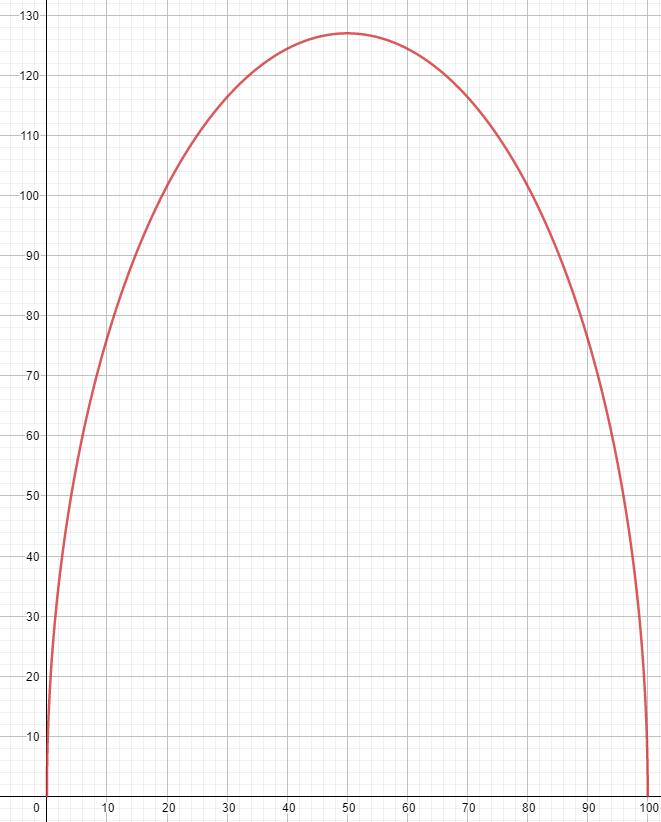
\includegraphics[scale=0.5]{images/geogebra-export.png}
\end{center}
\caption{Grafico del \({C^{'}}_{max}\) al variare di L}
\end{figure}

Le funzioni di membership e le regole della rete fuzzy sono state progettate sulla base di alcune situazioni che abbiamo individuato analizzando le coppie disturbate dei colori. Abbiamo notato che, a parità di DeltaE, la differenza delle coppie selezionate può essere percepita diversamente. Per questo motivo abbiamo individuato una serie di zone dello spazio LCh nella quale la percezione è diversa da quella specificata dal DeltaE.

\paragraph{Colori Insaturi} I colori poco saturi si distinguono con più difficoltà.
\paragraph{Colori Non Luminosi} I colori poco luminosi, similmente a quelli insaturi, non sono facilmente distinguibili.
\paragraph{Zona colori Arancione} I colori tendenti all'arancione sono più distinguibili.
\paragraph{Zona colori Giallo/Verde/Blu} I colori tendenti al giallo, al verde o al blu non sono facilmente distinguibili.

\section{Funzioni di Membership}
\begin{figure}[!ht]
\begin{center}
	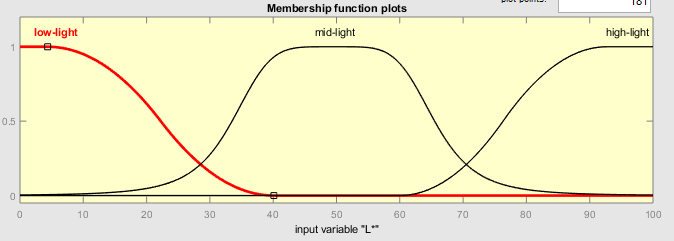
\includegraphics[scale=0.8]{images/rete2-membership-light.PNG}
\end{center}
\caption{Funzione di membership Light}
\end{figure}

\begin{figure}[!ht]
\begin{center}
	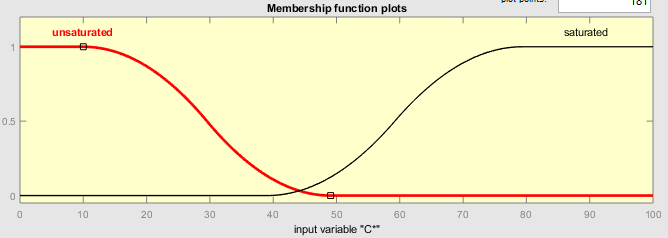
\includegraphics[scale=0.8]{images/rete2-membership-saturation.PNG}
\end{center}
\caption{Funzione di membership Saturation}
\end{figure}

\begin{figure}[!ht]
\begin{center}
	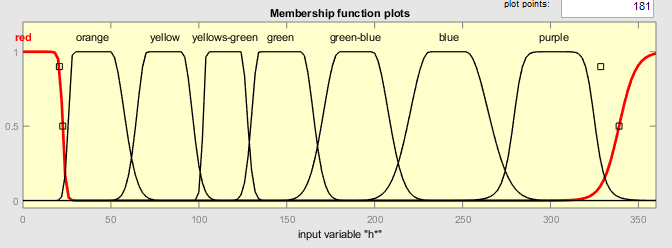
\includegraphics[scale=0.8]{images/rete2-membership-colors.PNG}
\end{center}
\caption{Funzione di membership Hue (Colore)}
\end{figure}

\begin{figure}[!ht]
\begin{center}
	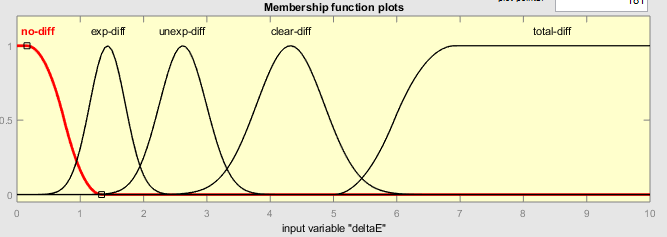
\includegraphics[scale=0.8]{images/rete2-membership-deltae.PNG}
\end{center}
\caption{Funzione di membership DeltaE (distanza euclidea)}
\end{figure}

\section{Regole}

\begin{table*}[!ht]
\centering
\begin{tabular}{|c c c c c c |}
\hline
L & c  & h & $\Delta E_{orig}$ & $\Delta E_{adj}$ & peso\\ \hline
-  & -           & -          & total-diff        & total-diff   & 0.2 \\ \hline
-  & -           & -          & clear-diff        & clear-diff   & 0.2 \\ \hline
-  & -           & -          & unexp-diff        & unexp-diff   & 0.2 \\ \hline
-  & -           & -          & exp-diff          & exp-diff   & 0.2 \\ \hline
-  & -           & -          & no-diff          & no-diff   & 0.2 \\ \hline
low-light  & -           & -          & total-diff        & exp-diff   & 1 \\ \hline
low-light  & -           & -          & clear-diff        & exp-diff   & 1 \\ \hline
low-light  & -           & -          & unexp-diff        & no-diff   & 1 \\ \hline
low-light  & -           & -          & exp-diff          & no-diff   & 1 \\ \hline
mid-light  & saturated   & orange     & unexp-diff        & exp-diff   & 1 \\ \hline
mid-light  & saturated   & green      & unexp-diff        & exp-diff   & 1 \\ \hline
mid-light  & saturated   & green      & exp-diff          & no-diff   & 1 \\ \hline
mid-light  & saturated   & blue       & clear-diff        & exp-diff   & 1 \\ \hline
high-light & saturated   & yellow     & unexp-diff        & no-diff   & 1 \\ \hline
high-light & saturated   & yellow     & clear-diff        & exp-diff   & 1 \\ \hline
not(low-light) & unsaturated & -      & not(no-diff)      & exp-diff   & 1 \\ \hline
not(low-light) & unsaturated & -      & no-diff           & no-diff   & 1 \\ \hline
\end{tabular}
\caption{Regole di inferenza del sistema Madamani}
\label{tab:rules}
\end{table*}